\section{Tugas 3 -- Segmentasi Pelanggan}
Data berisi 120.000 pelanggan dengan ringkasan perilaku 90 hari, tanpa label.

\subsection*{(a) Preprocessing}
\begin{itemize}
  \item \textbf{Skala dan skewness.} Variabel uang, hitungan, recency, dan aktivitas sangat menceng ke kanan (mis. \texttt{sesi\_per\_minggu} maks.\ 399,9)
        sehingga ditransformasi $\log(1+x)$, lalu di-\textit{winsorize} pada persentil 0,5--99,5 dan diskalakan dengan \textit{RobustScaler} (rentang persentil 10--90).
  \item \textbf{Data komposisional.} 16 porsi kategori dan 4 porsi waktu belanja masing-masing berjumlah 1; menaikkan satu porsi pasti menurunkan yang lain,
        sehingga jarak Euclidean pada porsi mentah tidak bermakna. Digunakan transformasi \textit{centered log-ratio}:
        $\mathrm{clr}(x)_i = \log(x_i+\varepsilon) - \frac{1}{D}\sum_j \log(x_j+\varepsilon)$, $\varepsilon = 10^{-3}$.
  \item \textbf{Kategorikal.} \texttt{kota\_tier} (ordinal 1--3) dipakai apa adanya; \texttt{perangkat} di-\textit{one-hot}.
  \item \textbf{Missing.} \texttt{rata2\_keranjang} kosong tepat ketika \texttt{frekuensi\_90h} = 0 (missing struktural), sehingga diisi 0 dan ditambah indikator \texttt{tidak\_aktif\_90h}.
  \item \textbf{Outlier dan inkonsistensi.} \texttt{rasio\_konversi} > 1 dan \texttt{belanja\_30h} > \texttt{belanja\_90h} dicatat sebagai inkonsistensi untuk tahap anomali (g).
\end{itemize}

\subsection*{(b) Seleksi dan pembobotan fitur}
\textbf{Kolom n01--n15.} Kamus data hanya menyebut n01--n10, tetapi data berisi 15 kolom. Korelasi Spearman maksimum dengan semua kolom lain hanya \TtigaNMaxKorelasi.
Namun kolom-kolom ini membentuk cluster yang sangat rapi \emph{di antara mereka sendiri} (silhouette \TtigaNSil) yang sama sekali tidak terkait
dengan cluster perilaku (ARI \TtigaNARIPerilaku), perangkat, maupun kota (Tabel~\ref{tab:t3_bukti_n}). Jika ikut dimasukkan, hasil clustering tertarik
ke struktur n (ARI dengan cluster n = \TtigaSemuaVsN; Tabel~\ref{tab:t3_konfigurasi_fitur}). Struktur yang kuat tetapi tidak berhubungan dengan perilaku
belanja tidak dapat ditindaklanjuti oleh tim marketing, sehingga n01--n15 dibuang.

\textbf{Redundansi dan bobot.} \texttt{belanja\_30h}/\texttt{frekuensi\_30h} berkorelasi tinggi dengan versi 90 harinya tetapi tetap dipakai sebagai sinyal tren terbaru.
Fitur dikelompokkan (RFM, kategori, waktu belanja, promo \& pembayaran, perilaku pasca-beli, aktivitas aplikasi, profil), dan setiap kolom diberi bobot
$1/\sqrt{n_{\text{kelompok}}}$ agar kelompok dengan banyak kolom (16 porsi kategori) tidak mendominasi jarak. Kepentingan tiap kelompok diukur dengan permutasi:
seberapa banyak label berubah jika kelompok diacak (Tabel~\ref{tab:t3_kepentingan_kelompok}); kelompok terpenting: \TtigaKelompokTerpenting.

\begin{table}[ht]
\centering\small
\begin{tabular}{p{0.75\linewidth}r}
\toprule
bukti & nilai \\
\midrule
max\_abs\_spearman\_n\_vs\_perilaku & 0.010 \\
max\_MI\_berlebih\_vs\_acuan\_acak & 0.025 \\
silhouette\_cluster\_n\_saja & 0.670 \\
ARI(cluster\_n, cluster\_perilaku) & -0.000 \\
ARI(cluster\_semua\_kolom, cluster\_n) & 0.083 \\
ARI(cluster\_semua\_kolom, cluster\_perilaku) & 0.398 \\
jumlah\_kolom\_n & 15.000 \\
ARI(cluster\_n, kota\_tier) & -0.000 \\
ARI(cluster\_n, perangkat) & -0.000 \\
\bottomrule
\end{tabular}
\caption{Bukti bahwa n01–n15 membentuk struktur sendiri yang tidak terkait perilaku/profil pelanggan.}
\label{tab:t3_bukti_n}
\end{table}

\begin{table}[ht]
\centering\small
\resizebox{\ifdim\width>\linewidth\linewidth\else\width\fi}{!}{%
\begin{tabular}{lrrrr}
\toprule
konfigurasi & n\_fitur & silhouette & stabilitas\_ARI & ARI\_dengan\_cluster\_n \\
\midrule
semua kolom termasuk n01–n15 & 62 & 0.079 & 0.706 & 0.083 \\
tanpa n, tanpa bobot & 47 & 0.085 & 0.746 & -0.000 \\
tanpa n, bobot per kelompok (dipakai) & 47 & 0.092 & 0.984 & -0.000 \\
\bottomrule
\end{tabular}
}
\caption{Konfigurasi fitur pada k=8: silhouette, stabilitas, dan seberapa jauh cluster ditarik oleh n01–n15.}
\label{tab:t3_konfigurasi_fitur}
\end{table}


\subsection*{(c)--(d) Metode dan jumlah cluster}
Kriteria untuk $k = 2,\dots,12$ (K-Means) ditunjukkan pada Gambar~\ref{fig:t3k} dan Tabel~\ref{tab:t3_kriteria_k}. Silhouette hampir datar (±0,09) dan BIC
terus turun, sehingga keduanya tidak dapat memilih $k$. Stabilitas (rata-rata ARI antar run subsampling 80\%) justru sangat informatif: hanya beberapa $k$
yang menghasilkan partisi konsisten. Aturan yang ditetapkan: \emph{$k$ terbesar dengan stabilitas $\geq 0{,}95$}. Terpilih $k = \TtigaK$
(stabilitas \TtigaStabK, sedangkan $k-1$: \TtigaStabKmin{} dan $k+1$: \TtigaStabKplus). Aturan ``terbesar'' dipilih karena
partisi stabil yang lebih rinci memisahkan kelompok yang benar-benar berbeda; salah satu cluster tambahan pada $k=\TtigaK$
ternyata kelompok berprofil bot yang kemudian diberi label $-1$ (butir g). Stabilitas memakai \texttt{n\_init} = 5 yang sama dengan model final.

Empat metode dibandingkan pada $k$ tersebut (Tabel~\ref{tab:t3_metode}): K-Means, Gaussian Mixture (kovarians diagonal), Agglomerative Ward
(sampel 15.000, sisanya di-assign ke centroid terdekat), dan HDBSCAN (menentukan jumlah cluster sendiri). Terpilih \textbf{\TtigaKonfigMetode}, metode
paling stabil antar seed. HDBSCAN hanya menemukan kelompok berkepadatan berbeda (pelanggan aktif vs tidak aktif) karena segmen lain tidak dipisahkan oleh celah kepadatan.

\begin{figure}[ht]\centering
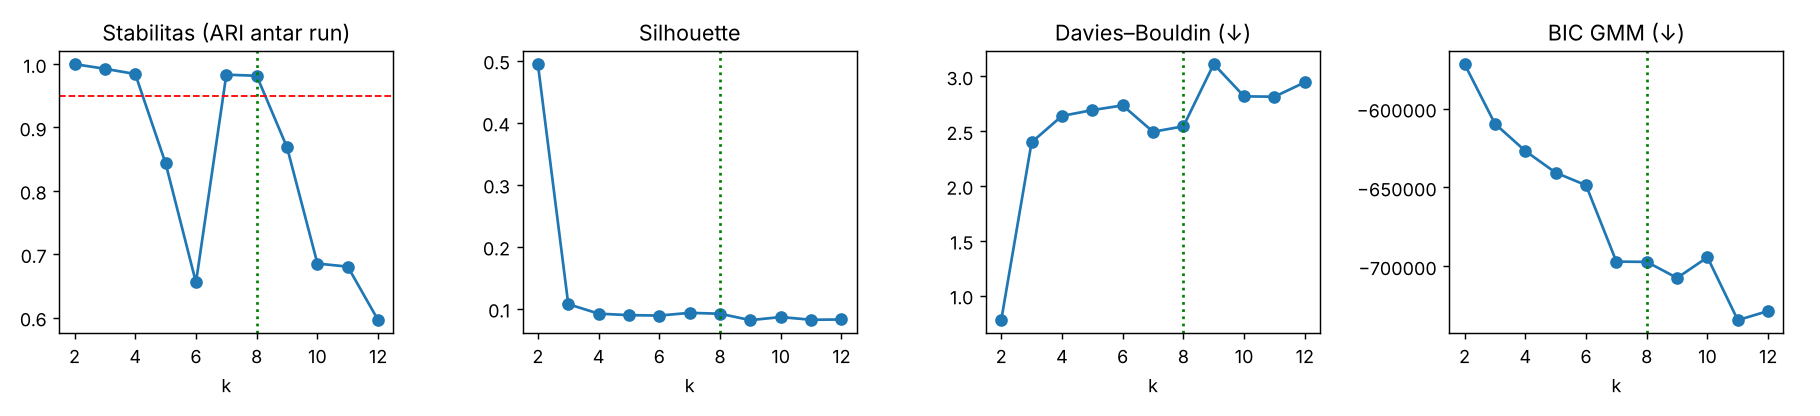
\includegraphics[width=\linewidth]{t3_kriteria_k.png}
\caption{Kriteria jumlah cluster; garis hijau = $k$ terpilih.}\label{fig:t3k}
\end{figure}
\begin{table}[ht]
\centering\small
\resizebox{\ifdim\width>\linewidth\linewidth\else\width\fi}{!}{%
\begin{tabular}{lrrrrrr}
\toprule
metode & n\_cluster & persen\_noise & silhouette & davies\_bouldin & ARI\_antar\_seed & ARI\_vs\_kmeans \\
\midrule
kmeans & 8 & 0.000 & 0.092 & 2.545 & 0.989 & 1.000 \\
gmm & 8 & 0.000 & 0.073 & 3.063 & 0.534 & 0.289 \\
agglomerative & 8 & 0.000 & 0.086 & 2.605 & 0.482 & 0.511 \\
hdbscan & 2 & 0.783 & 0.494 & 0.775 & 0.931 & 0.045 \\
\bottomrule
\end{tabular}
}
\caption{Perbandingan metode pada k=8 (HDBSCAN menentukan jumlah cluster sendiri).}
\label{tab:t3_metode}
\end{table}

